\documentclass[11pt]{article}
\usepackage[utf8]{inputenc}

%%%%%%%%%%%%%%%%%%%%%%%%%%%%%%%%%%%%%%%%%%%%%%%%%%%%%%%%%%%%%%%%
% PACKAGES, FORMATTING, LISTING, AND OTHER GRAPHICAL ELEMENTS  %
%%%%%%%%%%%%%%%%%%%%%%%%%%%%%%%%%%%%%%%%%%%%%%%%%%%%%%%%%%%%%%%%

\usepackage{amsmath,amssymb}
\usepackage[T1]{fontenc} % font encoding
\usepackage{graphicx} % for figures
\usepackage{float} % for figures
\usepackage{indentfirst} % indent first paragraph of section
\usepackage{soul,xcolor} % for colors
\usepackage{xkcdcolors} % colors from XKCD color survey
\usepackage{mathtools} % for boxed equations within \align
\usepackage{sectsty} % adjust section headers
\usepackage{fancyhdr} % page headers
\usepackage{titling} % reference title,author,date (in fancyhdr page header)
\usepackage{breqn} % automatically line wrap long Eqs.
\usepackage{pdfpages} % for \includepdf
\usepackage{pdflscape} % landscape 
\usepackage{mdframed} % for framed environment
\usepackage{listings} % for code blocks
\usepackage{inconsolata} % better monospace font
\usepackage{matlab-prettifier} % Better MATLAB listing highlighting
\usepackage[letterpaper, total={6.5in, 9in}]{geometry} % set paper and margin size
\usepackage{empheq} % multiline boxed equations, etc.
\usepackage{hyperref}
\usepackage{dsfont}	% gives you \mathds{} font
% \usepackage{enumerate} % custom enumerate numbering (or lettering in this case)
\usepackage[shortlabels]{enumitem} % more enumerate options
\usepackage{svg} % use inkscape to import svgs
\usepackage{bm} % bold symbols
\usepackage[parfill]{parskip} % replace indentation with paragraph spacing
\usepackage{dsfont} % gives you \mathds{} font

% hyperbolic trig inverse functions
\DeclareMathOperator{\sech}{sech}
\DeclareMathOperator{\csch}{csch}
\DeclareMathOperator{\arcsec}{arcsec}
\DeclareMathOperator{\arccot}{arcCot}
\DeclareMathOperator{\arccsc}{arcCsc}
\DeclareMathOperator{\arccosh}{arcCosh}
\DeclareMathOperator{\arcsinh}{arcsinh}
\DeclareMathOperator{\arctanh}{arctanh}
\DeclareMathOperator{\arcsech}{arcsech}
\DeclareMathOperator{\arccsch}{arcCsch}
\DeclareMathOperator{\arccoth}{arcCoth} 

% add page headers
\pagestyle{fancy}
\fancyhf{}
\fancyhead[LE,LO]{\thetitle}
\fancyhead[RE,RO]{\theauthor}
\fancyfoot[CE,CO]{\thepage}

% adjust section header font size
\sectionfont{\fontsize{20}{15}\selectfont}
\subsectionfont{\fontsize{14}{15}\selectfont}

% vertical table spacing
\renewcommand{\arraystretch}{1.5}

% right-side cases
% \newenvironment{rcases}
%     {\left.\begin{aligned}}
%     {\end{aligned}\right\rbrace}

% Multi-line \fbox
\newcommand\multilineBox[1]{
\noindent
\fbox{
	\parbox{0.97\linewidth}
		{#1}
	}
}

% number just one equation in an un-numbered align* environment
\newcommand\numberthis{\addtocounter{equation}{1}\tag{\theequation}}

%%%%%%%%%%%%%%%%%%%%%%%%%%%%%%%%%%%%%%%%%%%%%%%%%%%%%%%%%%%%%%%%

% set listings font to inconsolata
\DeclareFixedFont{\ttb}{T1}{txtt}{bx}{n}{9} % for bold
\DeclareFixedFont{\ttm}{T1}{txtt}{m}{n}{9}  % for normal

% general listings environment
\lstnewenvironment{code}
{\lstset{
    frame=single,
    % backgroundcolor=\color{xkcdPale},
    basicstyle=\fontfamily{pcr}\selectfont\tiny
    }}
{}

% MATLAB listings environment
\lstnewenvironment{MATLAB}
{\lstset{
    style=Matlab-editor,
    frame=single,
    % backgroundcolor=\color{xkcdPale},
    basicstyle=\fontfamily{pcr}\selectfont\tiny
    }}
{}

% Python style for listings
\newcommand\pythonstyle{\lstset{
    language=Python,
    basicstyle=\ttm,
    morekeywords={self},              % Add keywords here
    keywordstyle=\ttb\color{xkcdGreen},
    morekeywords=[2]{
        array,
        pi,
        zeros,
        max,
        sin,
        cos,
        linspace,
        size,
        plot,
        xlabel,
        title,
        legend,
        show,
        concatenate,
        logspace,
        exp,
        ylabel,
        savefig,
        grid,
        figure,
        axes
    },
    keywordstyle = [2]{\color{xkcdBrightBlue}},
    emph={__init__},                  % Custom highlighting
    emphstyle=\ttb\color{xkcdRed},    % Custom highlighting style
    stringstyle=\color{xkcdGreen},
    backgroundcolor=\color{xkcdPale},
    numberstyle=\color{xkcdGrey},
}}

% Python listings environment
\lstnewenvironment{python}[1][]
{\pythonstyle \lstset{#1}}
{}

% Python listings for external files
\newcommand\pythonexternal[2][]
{{\pythonstyle \lstinputlisting[#1]{#2}}}

% Python listings inline
\newcommand\pythoninline[1]{{\pythonstyle \lstinline!#1!}}


%%%%%%%%%%%%%%%%%%%%%%%%%%%%%%%%%%%%%%%%%%%%%%%%%%%%%%%%%%%%%%%%
% MATHEMATICAL SHORTCUTS                                       %
%%%%%%%%%%%%%%%%%%%%%%%%%%%%%%%%%%%%%%%%%%%%%%%%%%%%%%%%%%%%%%%%

% real and imaginary components
\renewcommand{\Re}{\operatorname{Re}}
\renewcommand{\Im}{\operatorname{Im}}

% Fourier transforms
\newcommand\fourier[1]{\frac{1}{\sqrt{2\pi}} \int_{-\infty}^\infty #1 e^{-i\omega x} \textrm{d}x}
\newcommand\inverseFourier[1]{\frac{1}{\sqrt{2\pi}} \int_{-\infty}^\infty #1 e^{i\omega x} \textrm{d}\omega}

% derivatives
\newcommand{\ppf}[2]{\frac{\partial #1}{\partial #2}}
\newcommand{\pppf}[3]{\frac{\partial^2 #1}{\partial #2 \partial #3}}
\newcommand{\ddf}[2]{\frac{\text{d} #1}{\text{d} #2}}
\newcommand{\DDf}[2]{\frac{\text{D} #1}{\text{D} #2}}

% norms
\newcommand\norm[1]{\lVert#1\rVert}

% statistical operators
\newcommand{\prob}{\operatorname{P}}
\newcommand{\expectation}{\operatorname{E}}
\newcommand{\variance}{\operatorname{Var}}
\newcommand{\stddev}{\operatorname{SD}}

% statistical distributions
\newcommand{\bernoulli}{\operatorname{Bernoulli}}
\newcommand{\binomial}{\operatorname{Binomial}}
\newcommand{\poisson}{\operatorname{Poisson}}
\newcommand{\normal}{\operatorname{Normal}}

%%%%%%%%%%%%%%%%%%%%%%%%%%%%%%%%%%%%%%%%%%%%%%%%%%%%%%%%%%%%%%%%
% COMMONLY USED COPYPASTAS
%%%%%%%%%%%%%%%%%%%%%%%%%%%%%%%%%%%%%%%%%%%%%%%%%%%%%%%%%%%%%%%%

% CODE BLOCK

% \begin{MATLAB}[caption={MATLAB script},label={code:p1}]
% for i = 1:n
%     disp('string')
% end
% \end{MATLAB}
% Code block \ref{code:p1}



% MULTIPLE EQUATIONS BOXED

% \begin{empheq}[box=\fbox]{align}
% \end{empheq}



% ENUMERTATE WITH a) instead of 1.

% \begin{enumerate}[label=\alph*)]
% \end{enumerate}
% 'Problem' sections
% \renewcommand{\thesection}{Part \arabic{section}}
\renewcommand{\thesubsection}{\arabic{section}.\alph{subsection}}
% \renewcommand{\thesubsection}{\arabic{subsection}}

\title{ENGR 510 Neural Networks Homework}
\author{Anthony Su}
\date{November 8, 2024}

\begin{document}
\thispagestyle{plain}
\maketitle


%%%%%%%%%%%%%%%%%%%%%%%%%%%%%%%%%%%%%%%%%%%%%%%%%%%%%%%%%%%%%%%%%%%%%%%%%%%%%%%%
% Understanding the Starter Code
%%%%%%%%%%%%%%%%%%%%%%%%%%%%%%%%%%%%%%%%%%%%%%%%%%%%%%%%%%%%%%%%%%%%%%%%%%%%%%%%
\subsection{}  % 1 -------------------------------------------------------------
\pythoninline{X} contains the digit image examples and \pythoninline{y} contains
the labels.

\subsection{}  % 2 -------------------------------------------------------------
70000 example images are loaded. They are each 28 pixels by 28 pixels in size.

\subsection{}  % 3 -------------------------------------------------------------
A 784-dimensional input layer is used because that is the dimension of the input
data, which consists of 784-pixel images. A 10-dimensional output layer is used
because that is the dimension of the output data, which consists of the
likelihood of the digits 0-9.

\subsection{}  % 4 -------------------------------------------------------------
The network has two hidden layers.

\subsection{}  % 5 -------------------------------------------------------------
There is a weight between each node in a layer and each node in the adjacent
layer. There are $784 \times 64 = 50176$ weights between the first and second
layers. There are $64 \times 32 = 2048$ weights between the second and third
layers. There are $32 \times 10 = 320$ weights between the third and fourth
layers. The total number of weights is $50176 + 2048 + 320 = 52544$

\subsection{}  % 6 -------------------------------------------------------------
\pythoninline{loss.backward()} computes the gradient and
\pythoninline{optimizer.step()} proceeds one step in the model optimization.
These are the commands which train the model in cell 6. In cell 7, the model is
being tested, not trained, so the model is only evaluated, not updated.

\subsection{}  % 7 -------------------------------------------------------------
$X=$ \pythoninline{images}

$Y=$ \pythoninline{pred}

$f=$ \pythoninline{model}

\pythoninline{model} also contains $\beta$ internally.

%%%%%%%%%%%%%%%%%%%%%%%%%%%%%%%%%%%%%%%%%%%%%%%%%%%%%%%%%%%%%%%%%%%%%%%%%%%%%%%%
% Understanding neural network architecture and training workflow
%%%%%%%%%%%%%%%%%%%%%%%%%%%%%%%%%%%%%%%%%%%%%%%%%%%%%%%%%%%%%%%%%%%%%%%%%%%%%%%%
\subsection{}  % 8 -------------------------------------------------------------
\begin{figure}[H]
    \centering
    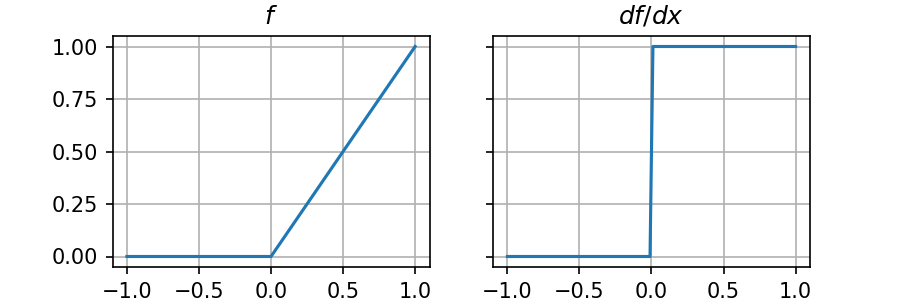
\includegraphics[width=4in]{8fig1.png}
    \caption{ReLU activation function}
    \label{8fig1}
\end{figure}
The derivative is queried many times when computing the gradient, and the
gradient is computed many times when fitting the model. Thus, an activation
function whose derivative is simple (piecewise constant in this case) makes
fitting the model much less expensive.

\subsection{}  % 9 -------------------------------------------------------------
The model's prediction is compared to the truth using the cross-entropy loss
function in line 37. Then, the gradient of the loss is computed using the
backpropagation algorithm in line 39. The model weights are then updated such as
to descend the gradient in line 40.

\subsection{}  % 10 ------------------------------------------------------------
The model is trained to accurately reproduce the outputs of the training data
set. However, the accuracy it achieves on the training data set does not
necessarily match the accuracy it achieves in general because the model
may have over-fitted to the training data set. Thus, data that was not used to
train the model is used for testing how the model generalizes.

\subsection{}  % 11 ------------------------------------------------------------
The model is slightly over-fit to the training data.

%%%%%%%%%%%%%%%%%%%%%%%%%%%%%%%%%%%%%%%%%%%%%%%%%%%%%%%%%%%%%%%%%%%%%%%%%%%%%%%%
% Modifying the neural network
%%%%%%%%%%%%%%%%%%%%%%%%%%%%%%%%%%%%%%%%%%%%%%%%%%%%%%%%%%%%%%%%%%%%%%%%%%%%%%%%
\subsection{}  % 12 ------------------------------------------------------------
\label{sec12}
\begin{python}[caption={Original Code},label={12code1}]
def my_model() -> nn.Module:
model = nn.Sequential(
    nn.Linear(784, 64),
    nn.ReLU(),
    nn.Linear(64, 32),
    nn.ReLU(),
    nn.Linear(32, 10),
)
return model
\end{python}

\begin{python}[caption={Modified Code},label={12code2}]
def my_model() -> nn.Module:
model = nn.Sequential(
    nn.Linear(784, 256),
    nn.ReLU(),
    nn.Linear(256, 10),
)
return model
\end{python}

The original model took 43 seconds to train on my CPU. The shallower model took
58 seconds to train on my CPU.

The original model has 52544 weights. The shallower model has 203264 weights.

%I would use the two-hidden-layer approach in the future because it achieves a
%similar test accuracy for a lower computational cost.

Since the single-hidden-layer architecture has a slightly higher accuracy on the
training data set and the increase in computational cost is small, I would
use that approach in the future. However, if the computational costs were orders
of magnitude higher, I would prefer the double-hidden-layer architecture for its
lower computational cost at similar levels of accuracy.

\subsection{}  % 13 ------------------------------------------------------------

Note: the model changes in Section \ref{sec12} were reverted before proceeding
with this section.

\begin{python}[caption={Original Code},label={13code1}]
optimizer = Adam(model.parameters(), lr=0.001)
\end{python}

\begin{python}[caption={Modified Code},label={13code2}]
optimizer = SGD(model.parameters(), lr=0.001)
\end{python}
I also imported the \pythoninline{SGD} class from the \pythoninline{torch.optim}
modeule.

The Adam optimization algorithm achieved a minimized loss of 0.12079 and an
accuracy of 96.918\% on the training data set. Its convergence is shown in
Figure \ref{13fig1}.

The SGD optimization algorithm achieved a minimized loss of 0.63998 and an
accuracy of 82.224\% on the training data set. Its convergence is shown in
Figure \ref{13fig2}.

\begin{figure}[H]
    \centering
    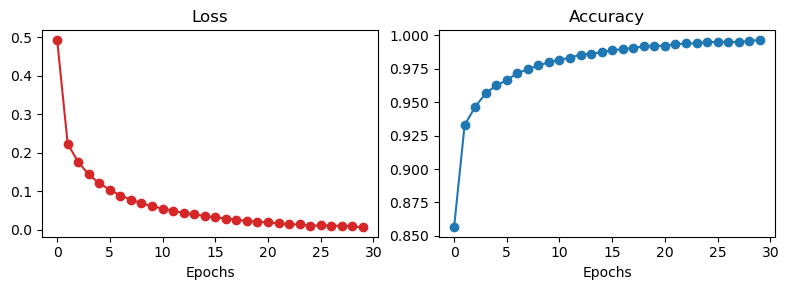
\includegraphics[width=5.5in]{13fig1.png}
    \caption{Convergence using Adam optimization algorithm}
    \label{13fig1}
\end{figure}
\begin{figure}[H]
    \centering
    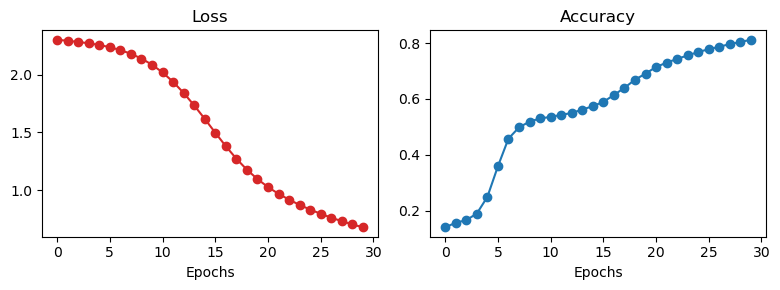
\includegraphics[width=5.5in]{13fig2.png}
    \caption{Convergence using SGD optimization algorithm}
    \label{13fig2}
\end{figure}

Adam converged with fewer epochs than SGD. In the context of iterative
algorithms, convergence refers to the state where further iterations do not
(significantly) further improve the quality of the answer.

\subsection{}  % 14 ------------------------------------------------------------

\begin{python}[caption={Original Code},label={14code1}]
optimizer = SGD(model.parameters(), lr=0.001)
\end{python}

\begin{python}[caption={ModifiedCode},label={14code2}]
optimizer = SGD(model.parameters(), lr=0.01)
\end{python}

With a learning rate of 0.001, the model achieved a minimized loss of 0.63998
and an accuracy of 82.224\% on the training data set. Its convergence is shown
in Figure \ref{14fig1}.

With a learning rate of 0.01, the model achieved a minimized loss of 0.18402
and an accuracy of 94.247\% on the training datat set. Its covergence is shown
in Figure \ref{14fig1}.

\begin{figure}[H]
    \centering
    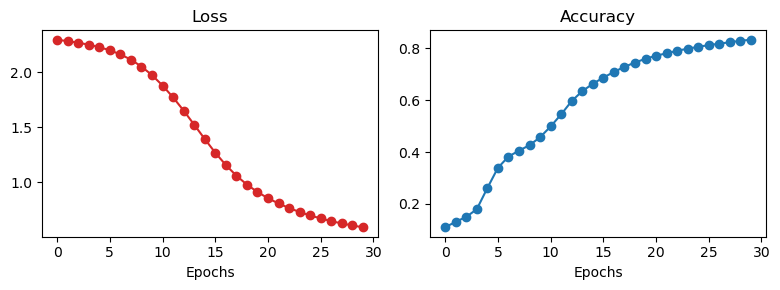
\includegraphics[width=5.5in]{14fig1.png}
    \caption{Convergence using learning rate of 0.001}
    \label{14fig1}
\end{figure}

\begin{figure}[H]
    \centering
    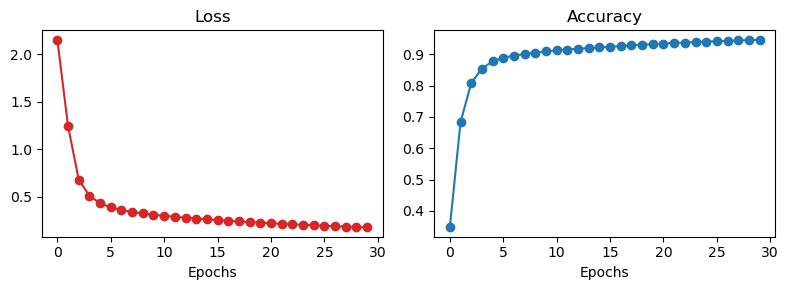
\includegraphics[width=5.5in]{14fig2.png}
    \caption{Convergence using learning rate of 0.01}
    \label{14fig2}
\end{figure}

The learning rate reduces convergence time, which increases the accuracy for a
given fixed training time or number of epochs. The possible pitfall of a higher
learning rate is the possibility of entirely skipping over minima.

\subsection{}  % 15 ------------------------------------------------------------

The purpose of this model is to predict which of ten classes an input most
probably belongs in. The cross-entropy loss function is defined in terms of
probability distributions and is well-suited to tuning the model to improve this
predictions of probability. In contrast, the mean squared error is defined in
for general quantities and does not accurately capture the meaning and
constraints inherent to probability.

\end{document}